\documentclass[t,aspectratio=169]{beamer}
%\usetheme{Madrid}
%\usecolortheme{default}
\usefonttheme{professionalfonts}
\setbeamertemplate{navigation symbols}{}
\setbeamertemplate{caption}[numbered]


\usepackage{bm}
\usepackage{soul}
\usepackage{tikz}
\usepackage{tikz-3dplot}
\usepackage{amsmath}
\usepackage{amsfonts}
\usepackage{amssymb}
\usepackage{booktabs}
\usepackage{array}
\usepackage{physics}
\usepackage{siunitx}
%\usepackage{graphicx}
\usepackage{multicol}
\usepackage{t1enc}
\usepackage[utf8]{inputenc}
\usepackage[magyar]{babel}
\usepackage{pgfplots}
\pgfplotsset{compat=1.18}

\usetikzlibrary{calc,3d,decorations.pathmorphing,decorations.pathreplacing,decorations.markings,snakes,arrows.meta,calc,patterns,angles,quotes,positioning,intersections}
\tikzset{snake it/.style={decorate, decoration=snake}}
% \usetheme{Madrid}
% \usecolortheme{whale}

\usepackage{hyperref}
\hypersetup{
    colorlinks=true,
    linkcolor=blue,
    filecolor=magenta,      
    urlcolor=cyan,
    pdftitle={(KTXFI1EBNF) Physics I. Lecture},
}


\newcommand{\E}{\mathbf{E}}
\newcommand{\B}{\mathbf{B}}
\newcommand{\Hf}{\mathbf{H}}
\newcommand{\J}{\mathbf{J}}
\newcommand{\Svec}{\mathbf{S}}
\newcommand{\kvec}{\mathbf{k}}
\newcommand{\rvec}{\mathbf{r}}
\newcommand{\ihat}{\hat{\mathbf{x}}}
\newcommand{\jhat}{\hat{\mathbf{y}}}
\newcommand{\khat}{\hat{\mathbf{z}}}

\tikzset{
  ray/.style={-Latex, thick, orange!80!black},
  axis/.style={-Latex, thick, black!70},
  lens/.style={draw=blue!70!black, fill=blue!12, very thick},
  mirror/.style={draw=gray!80!black, very thick},
  surface/.style={draw=black!70, thick},
  wave/.style={blue!70!black, thick, decorate, decoration={snake, amplitude=0.8mm, segment length=5mm}},
  screen/.style={draw=black!80, very thick},
  note/.style={font=\scriptsize, align=center}
}

% ----------------------------------------------------------------------------------------------------------------------------------------

\title{\includegraphics[width=45pt]{oepecsetlogo.png}\\(KTXFI1EBNF) Physics I. Lecture}

\author{Dr.~Gábor FACSKÓ, PhD\\\tiny Assistant Professor / Senior Research Fellow\\\textit{facsko.gabor@uni-obuda.hu}}

\institute{\Tiny Óbuda University, Faculty of Electrical Engineering, 1084 Budapest, Tavaszmező u. 17.\\Wigner Research Centre for Physics, Department of Space Physics and Space Technology, 1121 Budapest, Konkoly-Thege~Miklós~út~29–33.\\ \url{https://wigner.hu/~facsko.gabor}}

\date{April~27,~2026}

\logo{\includegraphics[height=0.9 true cm]{kekcsik.png}}

% ----------------------------------------------------------------------------------------------------------------------------------------

\begin{document}

\frame{\titlepage}

% ----------------------------------------------------------------------------------------------------------------------------------------

\begin{frame}
\frametitle{Current Updates and Announcements}
\begin{itemize}
\setlength{\parskip}{0pt}
\setlength{\itemsep}{4pt}
\item April 27, May 4, and go\dots
\item Homework No.~2 is now available. The deadline is May 4, 2026 at midnight.
\item Homework No.~3 will be available tonight. The deadline will be May 10, 2026 at midnight.
\end{itemize}
\end{frame}

% ----------------------------------------------------------------------------------------------------------------------------------------

\begin{frame}[fragile,squeeze,allowframebreaks]
\frametitle{Where are we?}
\begin{enumerate}
\setlength{\parskip}{0pt}
\setlength{\itemsep}{0pt}
\item \textbf{Mechanics I.:} Newton’s laws, equation of motion (review). Momentum. General concept of mechanical work, work theorem. Forms of mechanical energy.
\item \textbf{Mechanics II.:} Weight force, gravitational force, gravitational field. Work of the gravitational force. Conservative force field. Dissipative force field. Mechanical power.
\item \textbf{Mechanics of Rigid Bodies I.} Concept of a rigid body. Forces acting on a rigid body. Motion of a rigid body. Concept of the centre of mass. Location of the centre of mass. Torque. Angular momentum. Energy of a rotating rigid body, angular momentum of a rotating rigid body, Steiner’s theorem.
\item \textbf{Mechanics of Rigid Bodies II.} Principal theorems of rigid body motion; conservation laws. Collisions.
\item \textbf{Oscillations I.} Dynamic condition of harmonic oscillatory motion. Differential equation of harmonic undamped oscillatory motion.
\pagebreak
\item \textbf{Oscillations II.} Superposition of oscillations. Decomposition of oscillations into components. Damped oscillations. Forced oscillations, resonance. Coupled oscillations.
\item \textbf{Wave phenomena:} Reflection of waves, refraction of waves, diffraction of waves. Huygens–Fresnel principle. Interference of waves. Polarization of waves.
\item \textbf{Elements of acoustics:} Basics of acoustics. Fundamental concepts. Doppler effect. Sound intensity, loudness according to Weber–Fechner’s law.
\item \textbf{Thermodynamics I:} Temperature scales, thermal expansion, thermometers. State variables, ideal gas, state changes, ideal gas equation of state, Boyle’s law, Gay-Lussac’s laws, universal (combined) gas law, heat, specific heat, molar heat, heat capacity.
\item \textbf{Thermodynamics II:} Expansion work, internal energy, the first law of thermodynamics, forms of the first law in different state changes.
\pagebreak
\vskip -10 pt
\item \textbf{Thermodynamics III:} Cyclic processes, Carnot cycle, Carnot’s theorem, reduced heat, entropy, the second law of thermodynamics.
\item \textbf{Thermodynamics IV:} Kinetic theory of gases, molecular thermodynamics. Distributions, distribution functions. Elementary statistics.
\item \textbf{Electrostatics I.:} Electric charge: Fundamental electrical phenomena, electric charge and matter, Coulomb’s law (force between two point charges, unit of electric charge, permittivity of vacuum).
\item \textbf{Electrostatics II.:} The electric field: The electrostatic field (electric field strength, electric field lines). Determination of electric field strength. Gauss’s law (flux of the electric field). Electric field of a point charge.
\pagebreak
\item \textbf{Electrostatics III.:} Electrostatic potential: Work of the electric field (work done in an electric field). Electric potential (electrostatic potential). Electric potential difference, voltage. Electric potential of charge systems at small and large distances. Electrostatic energy.
\item \textbf{Elements of physical or wave optics.} \textit{Branches of optics. Light interference, light diffraction, diffraction through a slit, optical grating, light polarization. Light as an electromagnetic wave: Poynting vector. Optical instruments.}
\end{enumerate}
\end{frame}

% ----------------------------------------------------------------------------------------------------------------------------------------

% Slide 1: Fundamental Electrical Phenomena
\begin{frame}[fragile,squeeze,allowframebreaks]
\frametitle{Elements of physical and wave optics}
\begin{itemize}
\setlength{\parskip}{0pt}
\setlength{\itemsep}{4pt}
\item Branches of optics: When each model is useful?
\begin{table}
\small
\begin{tabular}{>{\bfseries}p{0.23\textwidth}p{0.35\textwidth}p{0.31\textwidth}}
\toprule
Branch & Main idea & Typical phenomena/instruments \\
\midrule
Geometrical optics & Light as rays; wavelength is negligible & Lenses, mirrors, cameras, microscopes \\
Wave optics & Light as a wave; phase matters & Interference, diffraction, coherence \\
%Physical optics & Wave model plus real boundaries and apertures & Diffraction by slits, gratings, imaging limits \\
%Electromagnetic optics & Light as coupled electric and magnetic fields & Polarization, energy flow, radiation pressure \\
%Quantum optics & Light as photons and quantum states & Photoelectric effect, lasers, single photons \\
\bottomrule
\end{tabular}
\end{table}
\item \textbf{Rule of thumb:} Ray optics works when object sizes and apertures are much larger than the wavelength. Wave effects dominate when path differences or apertures are comparable to $\lambda$.
  
\pagebreak
\item \textbf{Light as a wave: phase, amplitude, and intensity}
\begin{columns}[T]
\begin{column}{0.47\textwidth}
\item A monochromatic plane wave can be written as
\begin{eqnarray*}
  E(x,t)&=&E_0\cos(kx-\omega t+\phi),\\
  k&=&\frac{2\pi}{\lambda},\\
  \omega&=&2\pi f.
\end{eqnarray*}
\item In linear optical media, measured brightness is proportional to the time averaged square of the field:
\vskip -10 pt
$$I\sim \left\langle E^2\right\rangle_t.$$
\end{column}
\begin{column}{0.5\textwidth}
\vfill
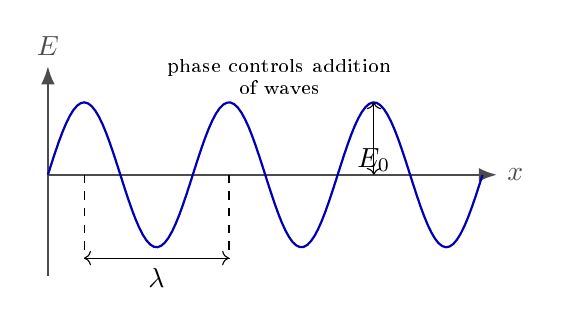
\begin{tikzpicture}[scale=0.92]
  \draw[axis] (0,0) -- (6.2,0) node[right] {$x$};
  \draw[axis] (0,-1.4) -- (0,1.5) node[above] {$E$};
  \draw[blue!70!black,thick,domain=0:6,samples=120] plot(\x,{sin(180*\x)});
  \draw[<->] (0.5,-1.15)--(2.5,-1.15) node[midway,below] {$\lambda$};
  \draw[dashed] (0.5,0)--(0.5,-1.15);
  \draw[dashed] (2.5,0)--(2.5,-1.15);
  \draw[<->] (4.5,0)--(4.5,1) node[midway,below] {$E_0$};
  \node[note] at (3.2,1.35) {phase controls addition\\of waves};
\end{tikzpicture}
\end{column}
\end{columns}

\pagebreak
\item \textbf{Two-source interference: path difference decides brightness}
\begin{columns}[T]
\begin{column}{0.49\textwidth}
\item Two coherent waves arriving at a point combine by superposition.
$$\delta = d\sin\theta,\qquad \Delta\phi=\frac{2\pi}{\lambda}\delta.$$
\item Constructive interference:
$$\delta=m\lambda \quad (m=0,\pm1,\pm2,\ldots).$$
\item Destructive interference:
\vskip -10 pt
$$ \delta=\left(m+\frac12\right)\lambda. $$
\end{column}
\begin{column}{0.48\textwidth}
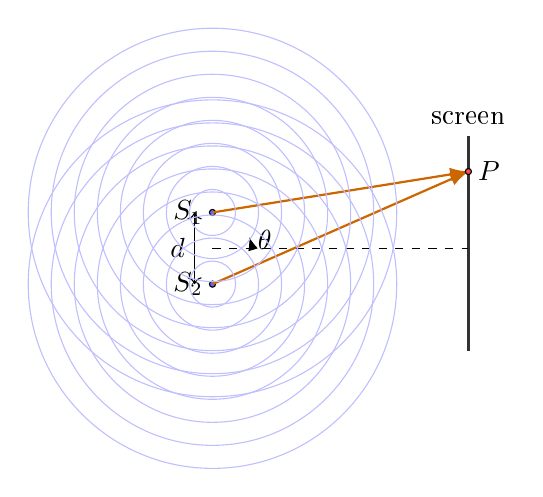
\begin{tikzpicture}[scale=0.65]
  \coordinate (S1) at (0,0.7);
  \coordinate (S2) at (0,-0.7);
  \coordinate (P) at (5,1.5);
  \draw[fill=blue!60] (S1) circle (0.06) node[left] {$S_1$};
  \draw[fill=blue!60] (S2) circle (0.06) node[left] {$S_2$};
  \draw[ray] (S1)--(P);
  \draw[ray] (S2)--(P);
  \draw[screen] (5,-2) -- (5,2.2) node[above]{screen};
  \draw[fill=red!70] (P) circle (0.06) node[right] {$P$};
  \draw[<->] (-0.35,-0.7)--(-0.35,0.7) node[midway,left] {$d$};
  \draw[dashed] (0,0)--(5,0);
  \draw[-Latex] (0.75,0) arc[start angle=0,end angle=17,radius=0.75];
  \node at (1.02,0.16) {$\theta$};
  \foreach \r in {0.45,0.9,1.35,1.8,2.25,2.7,3.15,3.6}{
    \draw[blue!25] (S1) circle (\r);
    \draw[blue!25] (S2) circle (\r);
  }
\end{tikzpicture}
\end{column}
\end{columns}

\pagebreak
\item \textbf{Interference intensity for equal amplitudes}
\begin{columns}[T]
\begin{column}{0.48\textwidth}
\item For two waves of equal amplitude,
$$E=E_0\cos\omega t+E_0\cos(\omega t+\Delta\phi),$$
so the intensity is
$$I=4I_0\cos^2\left(\frac{\Delta\phi}{2}\right).$$
\item The observable pattern is a map of phase differences.
\end{column}
\begin{column}{0.49\textwidth}
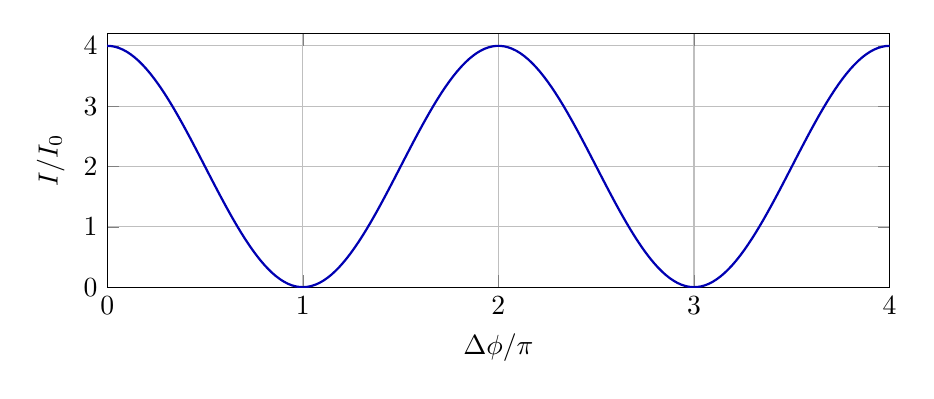
\begin{tikzpicture}
\begin{axis}[
  width=0.95\textwidth,height=4.8cm,
  xlabel={$\Delta\phi/\pi$},ylabel={$I/I_0$},
  xmin=0,xmax=4,ymin=0,ymax=4.2,
  xtick={0,1,2,3,4},ytick={0,1,2,3,4},
  grid=both]
\addplot[blue!70!black,thick,domain=0:4,samples=200] {4*cos(deg(pi*x/2))^2};
\end{axis}
\end{tikzpicture}
\end{column}
\end{columns}

\pagebreak
\item Diffraction: every aperture becomes a source of wavelets
\begin{columns}[T]
\begin{column}{0.47\textwidth}
\item \textbf{Huygens--Fresnel principle:} each point of a wavefront acts as a source of secondary spherical wavelets.

\vspace{0.5em}
\item Diffraction is strongest when
$$ a\sim \lambda,$$
where $a$ is the aperture or obstacle size.

\vspace{0.5em}
\item Wave optics explains why perfectly sharp shadows and unlimited resolution are impossible.
\end{column}
\begin{column}{0.5\textwidth}
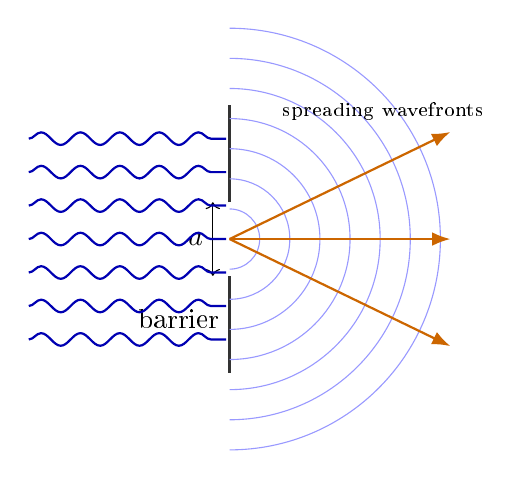
\begin{tikzpicture}[scale=0.85]
  \draw[screen] (0,-2) -- (0,-0.55);
  \draw[screen] (0,0.55) -- (0,2);
  \node[left] at (0,-1.2){barrier};
  \draw[<->] (-0.25,-0.55)--(-0.25,0.55) node[midway,left] {$a$};
  \foreach \y in {-1.5,-1.0,-0.5,0,0.5,1.0,1.5}{\draw[wave] (-3,\y)--(-0.05,\y);} 
  \foreach \r in {0.45,0.9,1.35,1.8,2.25,2.7,3.15}{\draw[blue!40] (0,\r) arc[start angle=90,end angle=-90,x radius=\r,y radius=\r];}
  \draw[ray] (0,0)--(3.3,1.6);
  \draw[ray] (0,0)--(3.3,0);
  \draw[ray] (0,0)--(3.3,-1.6);
  \node[note] at (2.3,1.9){spreading wavefronts};
\end{tikzpicture}
\end{column}
\end{columns}

\pagebreak
\item Fraunhofer diffraction: far-field geometry
\begin{columns}[T]
\begin{column}{0.48\textwidth}
\item Fraunhofer diffraction describes the far field, or the focal plane of a lens.

\item For a slit of width $a$, rays from different parts of the slit interfere at angle $\theta$.
$$ \Delta = a\sin\theta.$$
\item The minima occur when the aperture can be divided into canceling pairs:
  $$a\sin\theta=m\lambda, \qquad m=\pm1,\pm2,\ldots$$
\end{column}
\begin{column}{0.49\textwidth}
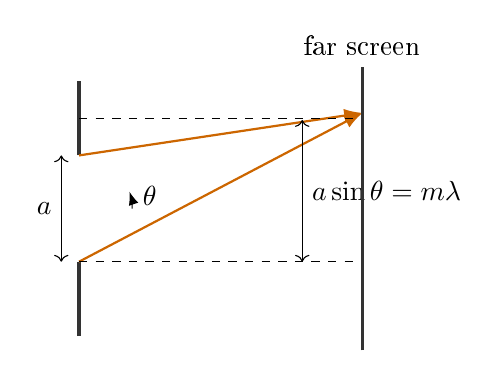
\begin{tikzpicture}[scale=0.9]
  \draw[screen] (0,-1.8)--(0,-0.75);
  \draw[screen] (0,0.75)--(0,1.8);
  \draw[<->] (-0.25,-0.75)--(-0.25,0.75) node[midway,left] {$a$};
  \coordinate (A) at (0,0.75);
  \coordinate (B) at (0,-0.75);
  \coordinate (P) at (4,1.35);
  \draw[ray] (A)--(P);
  \draw[ray] (B)--(P);
  \draw[dashed] (0,1.27)--(4,1.27);
  \draw[-Latex] (0.75,0) arc[start angle=0,end angle=18.6,radius=0.75];
  \node at (1.0,0.18) {$\theta$};
  \draw[dashed] (B)--($(B)+(4,0)$);
  \draw[<->] (3.15,-0.75)--(3.15,1.25) node[midway,right] {$a\sin\theta=m\lambda$};
  \draw[screen] (4,-2)--(4,2) node[above]{far screen};
\end{tikzpicture}
\end{column}
\end{columns}

\pagebreak
\item \textbf{Single-slit diffraction pattern}
\begin{columns}[T]
\begin{column}{0.43\textwidth}
\item For a uniformly illuminated slit,
\begin{eqnarray*}
I(\theta)&=&I_{\max}\left(\frac{\sin\beta}{\beta}\right)^2,\\
\beta&=&\frac{\pi a\sin\theta}{\lambda}.
 \end{eqnarray*}
Important features:
\begin{itemize}
  \item central maximum is the widest and brightest;
  \item dark fringes: $a\sin\theta=m\lambda$;
  \item increasing $a$ narrows the pattern.
  \end{itemize}
\end{column}
\begin{column}{0.54\textwidth}
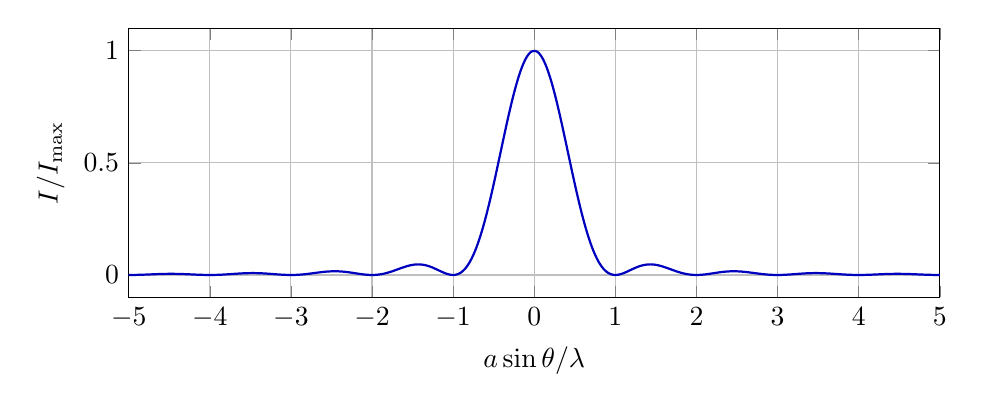
\begin{tikzpicture}
\begin{axis}[
  width=0.98\textwidth,height=5cm,
  xlabel={$a\sin\theta/\lambda$},ylabel={$I/I_{\max}$},
  xmin=-5,xmax=5,ymin=-0.1,ymax=1.1,
  grid=both]
\addplot[blue!75!black,thick,domain=-5:5,samples=500] {(x==0) ? 1 : (sin(deg(pi*x))/(pi*x))^2};
\end{axis}
\end{tikzpicture}
\end{column}
\end{columns}

\pagebreak
\item \textbf{Double slit: interference modulated by diffraction}
\begin{columns}[T]
\begin{column}{0.48\textwidth}
\item Real double slits have finite slit width $a$ and separation $d$.
$$ I(\theta)=I_{\max}\cos^2\left(\frac{\pi d\sin\theta}{\lambda}\right)
\left(\frac{\sin\beta}{\beta}\right)^2.$$
\item Interference fringes sit inside the single-slit diffraction envelope.
\end{column}
\begin{column}{0.49\textwidth}
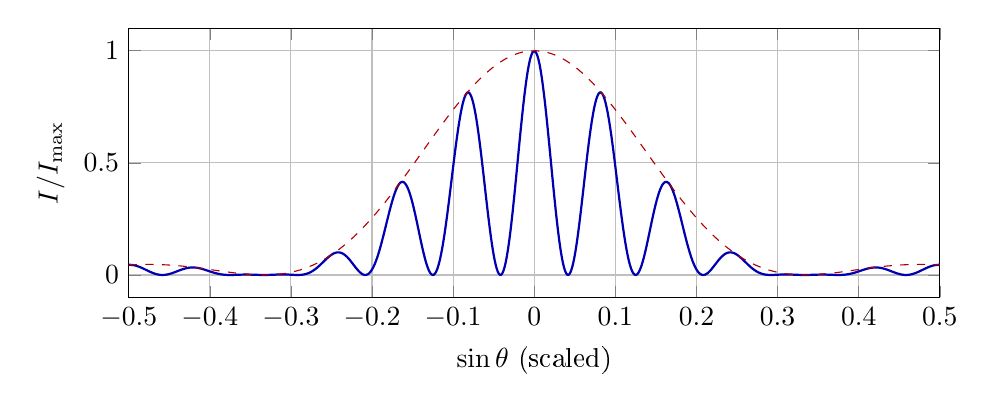
\begin{tikzpicture}
\begin{axis}[
  width=0.98\textwidth,height=5cm,
  xlabel={$\sin\theta$ (scaled)},ylabel={$I/I_{\max}$},
  xmin=-0.5,xmax=0.5,ymin=-0.1,ymax=1.1,
  grid=both]
\addplot[blue!70!black,thick,domain=-0.5:0.5,samples=700] {cos(deg(12*pi*x))^2*((x==0)?1:(sin(deg(3*pi*x))/(3*pi*x))^2)};
\addplot[red!70!black,dashed,domain=-0.5:0.5,samples=300] {((x==0)?1:(sin(deg(3*pi*x))/(3*pi*x))^2)};
\end{axis}
\end{tikzpicture}
\end{column}
\end{columns}

\pagebreak
\item \textbf{Optical grating: many slits sharpen the maxima}
\begin{columns}[T]
\begin{column}{0.47\textwidth}
\item For a grating with spacing $d$, principal maxima satisfy
\begin{eqnarray*} 
d\sin\theta&=&m\lambda,\\
m&=&0,\pm1,\pm2,\ldots
 \end{eqnarray*}
\item Because many slits interfere, the maxima become narrow and intense. This makes gratings useful for spectroscopy.
\end{column}
\begin{column}{0.5\textwidth}
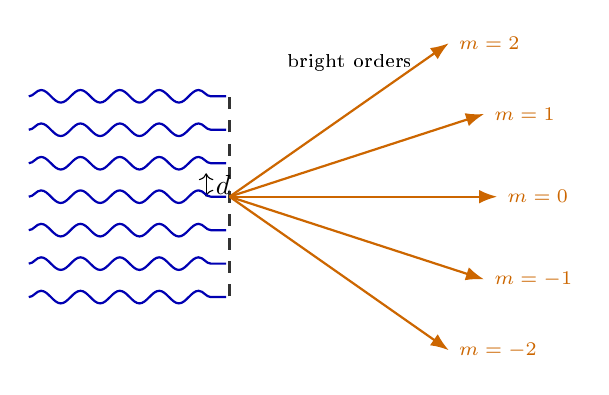
\begin{tikzpicture}[scale=0.85]
  \foreach \y in {-1.4,-1.05,-0.7,-0.35,0,0.35,0.7,1.05,1.4}{
    \draw[screen] (0,\y-0.09)--(0,\y+0.09);
  }
  \draw[<->] (-0.35,0)--(-0.35,0.35) node[midway,right] {$d$};
  \foreach \ang/\lab in {0/$m=0$,18/$m=1$,-18/$m=-1$,35/$m=2$,-35/$m=-2$}{
    \draw[ray] (0,0)--({4*cos(\ang)},{4*sin(\ang)}) node[right,note]{\lab};
  }
  \foreach \y in {-1.5,-1.0,-0.5,0,0.5,1.0,1.5}{\draw[wave] (-3,\y)--(-0.05,\y);} 
  \node[note] at (1.8,2.0){bright orders};
\end{tikzpicture}
\end{column}
\end{columns}

\pagebreak
\item \textbf{Grating dispersion and resolving power}
\begin{columns}[T]
\begin{column}{0.52\textwidth}
\item Different wavelengths leave at different angles:
$$d\sin\theta=m\lambda.$$
\item Angular dispersion:
$$\frac{d\theta}{d\lambda}=\frac{m}{d\cos\theta}.$$
\item Resolving power for $N$ illuminated grooves:
  $$R=\frac{\lambda}{\Delta\lambda}=mN.$$
\end{column}
\begin{column}{0.45\textwidth}
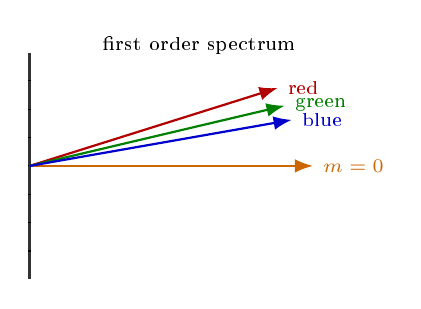
\begin{tikzpicture}[scale=0.9]
  \draw[screen] (0,-1.6)--(0,1.6);
  \foreach \y in {-1.2,-0.8,-0.4,0,0.4,0.8,1.2}{\draw (0.02,\y)--(-0.02,\y);} 
  \draw[ray] (0,0)--(4,0) node[right,note]{$m=0$};
  \draw[ray,red!70!black] (0,0)--(3.5,1.1) node[right,note]{red};
  \draw[ray,green!50!black] (0,0)--(3.6,0.85) node[right,note]{green};
  \draw[ray,blue!80!black] (0,0)--(3.7,0.65) node[right,note]{blue};
  \node[note] at (2.4,1.7){first order spectrum};
\end{tikzpicture}
\end{column}
\end{columns}

\pagebreak
\item \textbf{Polarization: direction of the electric field}
\begin{columns}[T]
\begin{column}{0.49\textwidth}
\item Polarization describes how the transverse electric field oscillates.
\begin{itemize}
  \item Linear: fixed direction.
  \item Circular: constant magnitude, rotating direction.
  \item Elliptical: general case.
\end{itemize}
\item For ideal polarizer axes separated by angle $\alpha$,
  $$ I=I_0\cos^2\alpha \quad \text{(Malus' law).}$$
\end{column}
\begin{column}{0.48\textwidth}
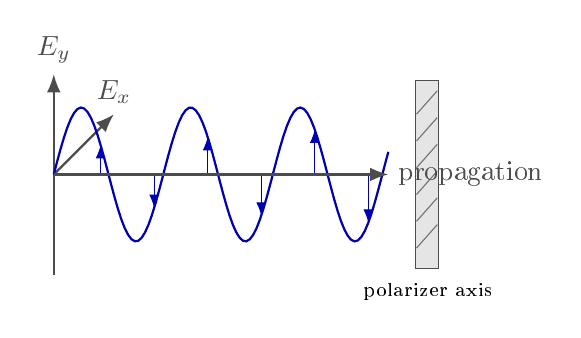
\begin{tikzpicture}[scale=0.85]
%  \draw[axis] (0,0)--(5,0) node[right]{propagation};
  \draw[axis] (0,-1.5)--(0,1.5) node[above]{$E_y$};
  \draw[axis] (0,0)--(0.9,0.9) node[above]{$E_x$};
  \draw[blue!70!black,thick,domain=0:5,samples=100] plot(\x,{sin(220*\x)});
  \foreach \x in {0.7,1.5,2.3,3.1,3.9,4.7}{\draw[blue!70!black,-Latex] (\x,0)--(\x,{sin(220*\x)});} 
  \draw[fill=gray!20,draw=black!70] (5.4,-1.4) rectangle (5.75,1.4);
  \foreach \y in {-1.1,-0.7,-0.3,0.1,0.5,0.9}{\draw[black!55] (5.42,\y)--(5.73,\y+0.35);} 
  \node[note] at (5.6,-1.75){polarizer axis};
    \draw[axis] (0,0)--(5,0) node[right]{propagation};
  \end{tikzpicture}
\end{column}
\end{columns}

\pagebreak
\item \textbf{How polarization is produced and used}
\begin{columns}[T]
\begin{column}{0.5\textwidth}
\item Common mechanisms:
\begin{itemize}
  \item selective absorption by polarizing filters;
  \item reflection near Brewster's angle;
  \item birefringence in anisotropic crystals;
  \item scattering by small particles.
\end{itemize}
Applications include LCDs, stress analysis, sunglasses, polarimetry, and astronomy.
\end{column}
\begin{column}{0.47\textwidth}
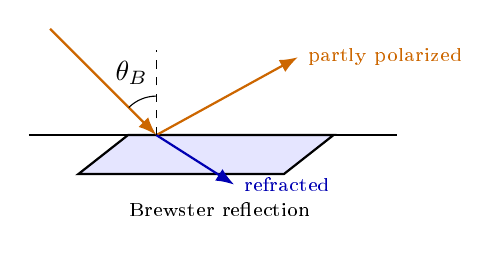
\begin{tikzpicture}[scale=0.9]
  \draw[thick] (-0.4,0)--(4.8,0);
  \draw[thick,fill=blue!10] (1,0)--(3.9,0)--(3.2,-0.55)--(0.3,-0.55)--cycle;
  \draw[ray] (-0.1,1.5)--(1.4,0);
  \draw[ray] (1.4,0)--(3.4,1.1) node[right,note]{partly polarized};
  \draw[ray,blue!70!black] (1.4,0)--(2.5,-0.7) node[right,note]{refracted};
  \draw[dashed] (1.4,0)--(1.4,1.2);
  \draw (1.4,0.55) arc[start angle=90,end angle=135,radius=0.55];
  \node at (1.05,0.88) {$\theta_B$};
  \node[note] at (2.3,-1.05){Brewster reflection};
\end{tikzpicture}
\end{column}
\end{columns}

\end{itemize}
\end{frame}

% ----------------------------------------------------------------------------------------------------------------------------------------


\begin{frame}[fragile,squeeze,allowframebreaks]
\frametitle{Electromagnetic waves}
\begin{itemize}
\setlength{\parskip}{0pt}
\setlength{\itemsep}{4pt}
\item \textbf{Maxwell equations in vacuum:} In a source-free vacuum,
\begin{eqnarray*}
\nabla\cdot\E&=&0,\\
\nabla\cdot\B&=&0,\\
\nabla\times\E&=&-\frac{\partial \B}{\partial t},\\
\nabla\times\B&=&\mu_0\epsilon_0\frac{\partial \E}{\partial t}.
\end{eqnarray*}
\item These equations imply that changing electric fields create magnetic fields, and changing magnetic fields create electric fields. A self-sustaining electromagnetic wave can propagate through empty space.

\item \textbf{Speed of light:} \hskip 80 pt $c=\frac{1}{\sqrt{\mu_0\epsilon_0}}.$

\pagebreak
\item \textbf{Derivation of the EM wave equation for $\mathbf{E}$}
\begin{itemize}
\item Take the curl of Faraday's law:
  $$\nabla\times(\nabla\times\E)=-\frac{\partial}{\partial t}(\nabla\times\B).$$
\item Use the vector identity
$$\nabla\times(\nabla\times\E)=\nabla(\nabla\cdot\E)-\nabla^2\E.$$
\item In vacuum, $\nabla\cdot\E=0$, so
  $$ -\nabla^2\E=-\frac{\partial}{\partial t}\left(\mu_0\epsilon_0\frac{\partial \E}{\partial t}\right).$$

\pagebreak
\item Therefore
$$\boxed{\nabla^2\E=\mu_0\epsilon_0\frac{\partial^2\E}{\partial t^2}}
\qquad \Longleftrightarrow \qquad
\boxed{\nabla^2\E-\frac{1}{c^2}\frac{\partial^2\E}{\partial t^2}=0.}$$
\end{itemize}

\pagebreak
\item \textbf{Derivation of the EM wave equation for $\mathbf{B}$}
\begin{itemize}
\item Take the curl of Ampere--Maxwell's law:
$$\nabla\times(\nabla\times\B)=\mu_0\epsilon_0\frac{\partial}{\partial t}(\nabla\times\E).$$
\item Use $\nabla\cdot\B=0$ and Faraday's law:
  $$ -\nabla^2\B=\mu_0\epsilon_0\frac{\partial}{\partial t}\left(-\frac{\partial\B}{\partial t}\right).$$
\item Thus
$$\boxed{\nabla^2\B=\mu_0\epsilon_0\frac{\partial^2\B}{\partial t^2}}
\qquad \Longleftrightarrow \qquad
\boxed{\nabla^2\B-\frac{1}{c^2}\frac{\partial^2\B}{\partial t^2}=0.}$$

\pagebreak
\item Plane-wave solutions satisfy
$$ \E\perp\B\perp\kvec,\qquad B_0=\frac{E_0}{c}.$$
\end{itemize}

\pagebreak
\item \textbf{Relation Between the Electric and Magnetic Fields}
\begin{itemize}
\item Assume similarly that
$$\mathbf B(\mathbf r,t)=\mathbf B_0e^{i(\mathbf k\cdot \mathbf r-\omega t)}.$$

\item Using Faraday's law,
$$\nabla\times \mathbf E=-\frac{\partial \mathbf B}{\partial t},$$
we obtain
$$i\mathbf k\times \mathbf E=i\omega \mathbf B.$$

\item Hence
  $$\boxed{\mathbf B=\frac{1}{\omega}\mathbf k\times \mathbf E}$$

\pagebreak
and, since \(\omega=ck\),
$$\boxed{B_0=\frac{E_0}{c}}\qquad\text{or}\qquad\boxed{\frac{E_0}{B_0}=c.}$$

\item The plane electromagnetic wave is transverse:
$$\boxed{\mathbf k\perp \mathbf E,\qquad\mathbf k\perp \mathbf B,\qquad\mathbf E\perp \mathbf B.}$$
\end{itemize}

\pagebreak
\item \textbf{Plane Electromagnetic Wave:} A real physical plane-wave solution may be written as
\vskip -10 pt
$$\mathbf E(\mathbf r,t)=\mathbf E_0 \cos(\mathbf k\cdot\mathbf r-\omega t),$$
\vskip -10 pt
and
\vskip -20 pt
$$\mathbf B(\mathbf r,t)=\frac{1}{\omega}\mathbf k\times \mathbf E_0\cos(\mathbf k\cdot\mathbf r-\omega t).$$

\begin{center}
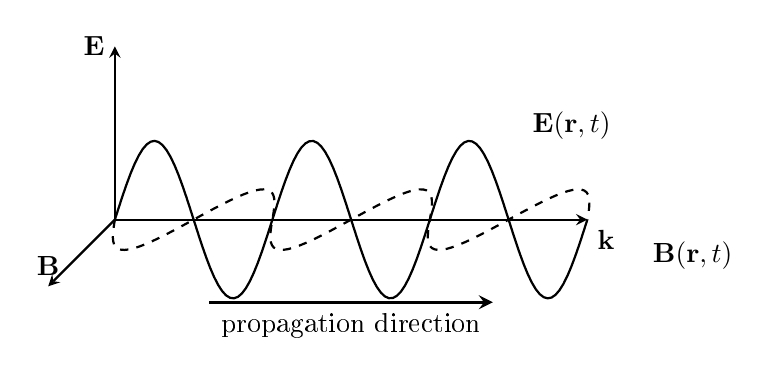
\begin{tikzpicture}[scale=1.0, >=stealth]

% axes
\draw[->, thick] (0,0,0) -- (6,0,0) node[below right] {$\mathbf k$};
\draw[->, thick] (0,0,0) -- (0,2.2,0) node[left] {$\mathbf E$};
\draw[->, thick] (0,0,0) -- (0,0,2.2) node[above] {$\mathbf B$};

% wave along x, E along y
\draw[domain=0:6, samples=120, thick]
plot ({\x},{1.0*sin(180*\x)},0);

% wave along x, B along z
\draw[domain=0:6, samples=120, thick, dashed]
plot ({\x},0,{1.0*sin(180*\x)});

% labels
\node at (5.8,1.2,0) {$\mathbf E(\mathbf r,t)$};
\node at (7.8,0,1.2) {$\mathbf B(\mathbf r,t)$};

% propagation arrow
\draw[->, very thick] (1.2,-1.05,0) -- (4.8,-1.05,0)
node[midway, below] {propagation direction};

\end{tikzpicture}
\end{center}

\pagebreak
\item \textbf{Plane electromagnetic wave and the Poynting vector}
\begin{columns}[T]
  \begin{column}{0.48\textwidth}
\begin{itemize}
\item For a plane wave moving in $+z$,
\begin{eqnarray*}
\E&=&E_0\cos(kz-\omega t)\,\ihat,\\
\B&=&B_0\cos(kz-\omega t)\,\jhat.
 \end{eqnarray*}
\item The energy flux density is the Poynting vector:
$$\boxed{\Svec=\frac{1}{\mu_0}\E\times\B.}$$
\item For a plane wave,
  $$\langle S\rangle=\frac{1}{2}\epsilon_0 c E_0^2.$$
\end{itemize}
\end{column}
\begin{column}{0.49\textwidth}
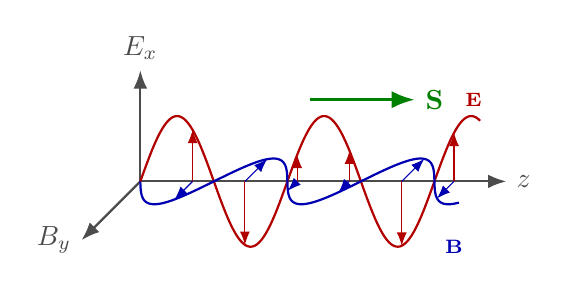
\begin{tikzpicture}[scale=0.83]
  \draw[axis] (0,0)--(5.6,0) node[right]{$z$};
  \draw[axis] (0,0)--(0,1.7) node[above]{$E_x$};
  \draw[axis] (0,0)--(-0.9,-0.9) node[left]{$B_y$};
  \draw[red!70!black,thick,domain=0:5.2,samples=150] plot(\x,{1.0*sin(160*\x)});
  \draw[blue!70!black,thick,domain=0:5.2,samples=150] plot({\x-0.35*sin(160*\x)},{-0.35*sin(160*\x)});
  \foreach \x in {0.8,1.6,2.4,3.2,4.0,4.8}{
    \draw[red!70!black,-Latex] (\x,0)--(\x,{sin(160*\x)});
    \draw[blue!70!black,-Latex] (\x,0)--({\x-0.35*sin(160*\x)},{-0.35*sin(160*\x)});
  }
  \draw[-Latex,very thick,green!50!black] (2.6,1.25)--(4.2,1.25) node[right]{$\Svec$};
  \node[red!70!black,note] at (5.1,1.25){$\E$};
  \node[blue!70!black,note] at (4.8,-1.0){$\B$};
\end{tikzpicture}
\end{column}
\end{columns}

\pagebreak
\item \textbf{Energy density and radiation pressure}
\begin{itemize}
\item The electromagnetic energy density is
$$ u=\frac{1}{2}\epsilon_0 E^2+\frac{1}{2\mu_0}B^2.$$
\item For a plane wave the electric and magnetic contributions are equal, so
$$u=\epsilon_0 E^2=\frac{B^2}{\mu_0}.$$
\item The Poynting vector gives energy crossing unit area per unit time:
  $$\Svec=u\,c\,\hat{\mathbf{k}} \quad \text{for a plane wave.}$$

\pagebreak
\item Radiation pressure follows from momentum transport:
$$p_{\text{absorber}}=\frac{I}{c},
\qquad
p_{\text{mirror}}=\frac{2I}{c}.$$
\end{itemize}

\end{itemize}

\end{frame}

% ----------------------------------------------------------------------------------------------------------------------------------------

\begin{frame}[fragile,squeeze,allowframebreaks]
\frametitle{Optical instruments: lenses and mirrors}
\begin{itemize}
\setlength{\parskip}{0pt}
\setlength{\itemsep}{4pt}
\begin{columns}[T]
\begin{column}{0.48\textwidth}
\item Optical instruments form images by controlling wavefronts.
\begin{itemize}
  \item Lenses refract light.
  \item Mirrors reflect light.
  \item Stops and apertures control brightness and resolution.
  \item Detector or eye records the final image.
\end{itemize}
For thin lenses and spherical mirrors:
$$\frac{1}{f}=\frac{1}{s_o}+\frac{1}{s_i},\qquad m=-\frac{s_i}{s_o}.$$
\end{column}
\begin{column}{0.49\textwidth}
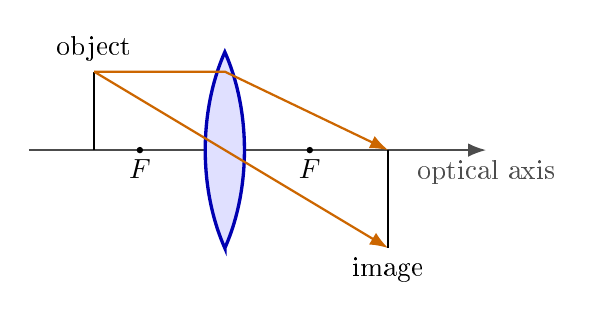
\begin{tikzpicture}[scale=0.83]
  \draw[axis] (-3,0)--(4,0) node[below]{optical axis};
  \draw[lens] (0,-1.5) .. controls (0.4,-0.6) and (0.4,0.6) .. (0,1.5) .. controls (-0.4,0.6) and (-0.4,-0.6) .. cycle;
  \draw[thick] (-2,0)--(-2,1.2) node[above]{object};
  \draw[ray] (-2,1.2)--(0,1.2)--(2.5,0);
  \draw[ray] (-2,1.2)--(0,0)--(2.5,-1.5);
  \draw[thick] (2.5,0)--(2.5,-1.5) node[below]{image};
  \draw[fill=black] (-1.3,0) circle (0.04) node[below]{$F$};
  \draw[fill=black] (1.3,0) circle (0.04) node[below]{$F$};
\end{tikzpicture}
\end{column}
\end{columns}

\pagebreak
\item \textbf{Convex and concave lenses}
\begin{columns}[T]
\begin{column}{0.5\textwidth}
\textbf{Convex lens:} converging. Parallel rays focus at the real focal point.
\begin{center}
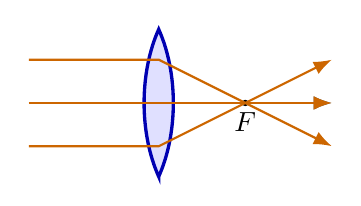
\begin{tikzpicture}[scale=0.55]
  \draw[axis] (-3,0)--(4,0);
  \draw[lens] (0,-1.7) .. controls (0.45,-0.7) and (0.45,0.7) .. (0,1.7) .. controls (-0.45,0.7) and (-0.45,-0.7) .. cycle;
  \draw[fill=black] (2,0) circle (0.06) node[below]{$F$};
  \foreach \y in {-1,0,1}{\draw[ray] (-3,\y)--(0,\y)--(2,0)--(4,-\y);} 
\end{tikzpicture}
\end{center}
$$f>0$$
\end{column}
\begin{column}{0.5\textwidth}
\textbf{Concave lens:} diverging. Parallel rays appear to come from a virtual focal point.
\begin{center}
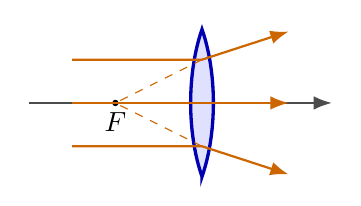
\begin{tikzpicture}[scale=0.55]
  \draw[axis] (-4,0)--(3,0);
  \draw[lens] (0,-1.7) .. controls (-0.35,-0.7) and (-0.35,0.7) .. (0,1.7) .. controls (0.35,0.7) and (0.35,-0.7) .. cycle;
  \draw[fill=black] (-2,0) circle (0.06) node[below]{$F$};
  \foreach \y in {-1,0,1}{
    \draw[ray] (-3,\y)--(0,\y)--(2,{1.65*\y});
    \draw[dashed,orange!80!black] (0,\y)--(-2,0);
  }
\end{tikzpicture}
\end{center}
$$f<0$$
\end{column}
\end{columns}

\pagebreak
\item \textbf{Convex and concave spherical mirrors}
\begin{columns}[T]
\begin{column}{0.5\textwidth}
\textbf{Concave spherical mirror:} converging; real focus in front of mirror.
\begin{center}
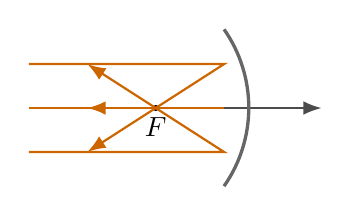
\begin{tikzpicture}[scale=0.62]
  \draw[axis] (-4,0)--(2,0);
  \draw[mirror] (0,-1.6) arc (-35:35:2.8);
  \draw[fill=black] (-1.4,0) circle (0.05) node[below]{$F$};
  \foreach \y in {-0.9,0,0.9}{\draw[ray] (-4,\y)--(0,\y)--(-1.4,0)--(-2.8,-\y);} 
\end{tikzpicture}
\end{center}
\end{column}
\begin{column}{0.5\textwidth}
\textbf{Convex spherical mirror:} diverging; virtual focus behind mirror.
\begin{center}
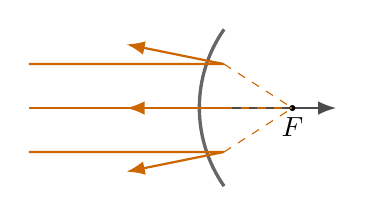
\begin{tikzpicture}[scale=0.62]
  \draw[axis] (-4,0)--(2.3,0);
  \draw[mirror] (0,-1.6) arc (215:145:2.8);
  \draw[fill=black] (1.4,0) circle (0.05) node[below]{$F$};
  \foreach \y in {-0.9,0,0.9}{
    \draw[ray] (-4,\y)--(0,\y)--(-2,{1.45*\y});
    \draw[dashed,orange!80!black] (0,\y)--(1.4,0);
  }
\end{tikzpicture}
\end{center}
Convex mirrors give a wide field of view but virtual, reduced images.
\end{column}
\end{columns}

\pagebreak
\item \textbf{Concave parabolic mirror}
\begin{columns}[T]
  \begin{column}{0.45\textwidth}
\begin{itemize}
\item A parabolic mirror focuses parallel incoming rays to one point without spherical aberration:
$$ y^2=4fx. $$
\item It is ideal for on-axis astronomical telescopes and searchlights.
\end{itemize}
\end{column}
\begin{column}{0.52\textwidth}
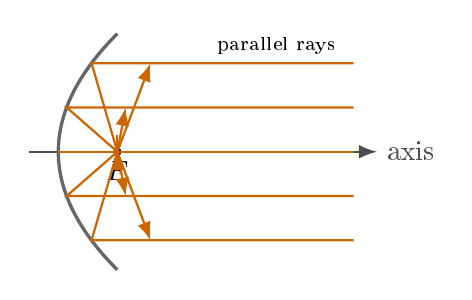
\begin{tikzpicture}[scale=0.75]
  \draw[axis] (-0.5,0)--(5.4,0) node[right]{axis};
  \draw[mirror,domain=-2:2,samples=100] plot({0.25*\x*\x},{\x});
  \draw[fill=black] (1,0) circle (0.06) node[below]{$F$};
  \foreach \y in {-1.5,-0.75,0,0.75,1.5}{
    \pgfmathsetmacro{\xhit}{0.25*\y*\y}
    \draw[ray] (5,\y)--(\xhit,\y)--(1,0)--(1+\xhit,-\y);
  }
  \node[note] at (3.7,1.8){parallel rays};
\end{tikzpicture}
\end{column}
\end{columns}

\pagebreak
\item \textbf{Concave hyperbolic mirror}
\begin{columns}[T]
  \begin{column}{0.48\textwidth}
\begin{itemize}
\item A hyperbolic mirror has two foci. A ray directed toward one focus reflects as if it came from the other focus.

\item This property is used in Cassegrain and Ritchey--Chretien telescopes, where a convex hyperbolic secondary redirects light through the primary mirror.
\end{itemize}
\end{column}
\begin{column}{0.49\textwidth}
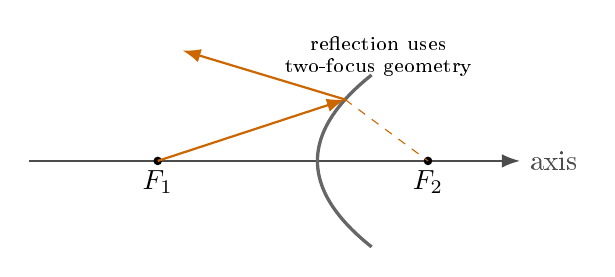
\begin{tikzpicture}[scale=0.78]
  \draw[axis] (-3.5,0)--(4.5,0) node[right]{axis};
  \draw[mirror,domain=-1.4:1.4,samples=100] plot({1.2+0.45*\x*\x},{\x});
  \draw[fill=black] (-1.4,0) circle (0.06) node[below]{$F_1$};
  \draw[fill=black] (3.0,0) circle (0.06) node[below]{$F_2$};
  \coordinate (P) at (1.65,1.0);
  \draw[ray] (-1.4,0)--(P);
  \draw[ray] (P)--(-1.0,1.8);
  \draw[dashed,orange!80!black] (P)--(3,0);
  \node[note] at (2.2,1.7){reflection uses\\two-focus geometry};
\end{tikzpicture}
\end{column}
\end{columns}

\end{itemize}
\end{frame}

% ----------------------------------------------------------------------------------------------------------------------------------------


\begin{frame}[fragile,squeeze,allowframebreaks]
\frametitle{Optical instruments: telescopes}
\begin{itemize}
\setlength{\parskip}{0pt}
\setlength{\itemsep}{4pt}
\item \textbf{Galilean telescope: upright image, short tube}
\begin{columns}[T]
\begin{column}{0.47\textwidth}
\item \textbf{Objective:} convex lens.\newline
\item \textbf{Eyepiece:} concave lens placed before the real focal point of the objective.

\item For relaxed eye viewing, approximately:
$$ L=f_o-|f_e|,\qquad M=-\frac{f_o}{f_e}>0. $$
\item It gives an upright image, but the field of view is narrow.
  \end{column}
\begin{column}{0.5\textwidth}
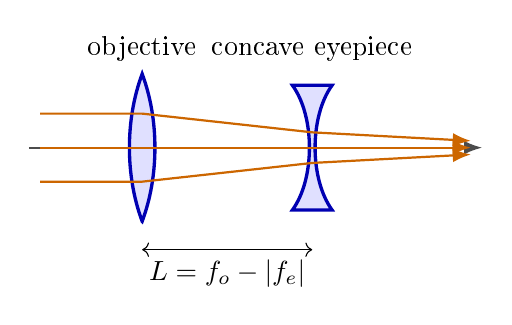
\begin{tikzpicture}[scale=0.72]
  \draw[axis] (-1,0)--(7,0);
  \draw[lens] (1,-1.3) .. controls (1.3,-0.5) and (1.3,0.5) .. (1,1.3) .. controls (0.7,0.5) and (0.7,-0.5) .. cycle;
\draw[lens]  (3.65,-1.1) .. controls (4.05,-0.55) and (4.05,0.55) .. (3.65,1.1) -- (4.35,1.1) .. controls (3.95,0.55) and (3.95,-0.55) .. (4.35,-1.1)  -- cycle;
  \node[above] at (1,1.35){objective};
  \node[above] at (4,1.35){concave eyepiece};
  \foreach \y in {-0.6,0,0.6}{\draw[ray] (-0.8,\y)--(1,\y)--(4,{0.45*\y})--(6.8,{0.2*\y});}
  \draw[<->] (1,-1.8)--(4,-1.8) node[midway,below]{$L=f_o-|f_e|$};
\end{tikzpicture}
\end{column}
\end{columns}

\pagebreak
\item \textbf{Keplerian telescope: real intermediate image}
\begin{columns}[T]
\begin{column}{0.47\textwidth}
\item \textbf{Objective:} convex lens.\newline
\item \textbf{Eyepiece:} convex lens.

\item For relaxed viewing:
$$ L=f_o+f_e, \qquad M=-\frac{f_o}{f_e}.$$
\item The image is inverted, but the field of view is wider and the intermediate image plane can hold a reticle or detector.
\end{column}
\begin{column}{0.5\textwidth}
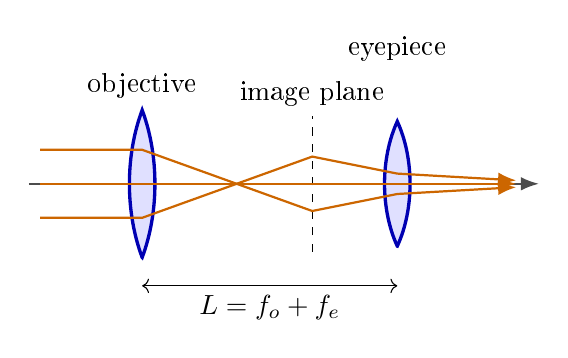
\begin{tikzpicture}[scale=0.72]
  \draw[axis] (-1,0)--(8,0);
  \draw[lens] (1,-1.3) .. controls (1.3,-0.5) and (1.3,0.5) .. (1,1.3) .. controls (0.7,0.5) and (0.7,-0.5) .. cycle;
  \draw[lens] (5.5,-1.1) .. controls (5.8,-0.45) and (5.8,0.45) .. (5.5,1.1) .. controls (5.2,0.45) and (5.2,-0.45) .. cycle;
  \node[above] at (1,1.35){objective};
  \node[above] at (5.5,2.0){eyepiece};
  \draw[dashed] (4, -1.2)--(4,1.2) node[above]{image plane};
  \foreach \y in {-0.6,0,0.6}{\draw[ray] (-0.8,\y)--(1,\y)--(4,{-0.8*\y})--(5.5,{-0.3*\y})--(7.6,{-0.1*\y});}
  \draw[<->] (1,-1.8)--(5.5,-1.8) node[midway,below]{$L=f_o+f_e$};
\end{tikzpicture}
\end{column}
\end{columns}

\pagebreak
\item \textbf{Newtonian reflector}
\begin{columns}[T]
\begin{column}{0.47\textwidth}
\item A concave primary mirror forms a focus. A flat secondary mirror redirects the beam sideways to an eyepiece.

\item \textbf{Strengths:} simple, economical, no chromatic aberration.\newline
\item \textbf{Limits:} off-axis coma and central obstruction.
\end{column}
\begin{column}{0.5\textwidth}
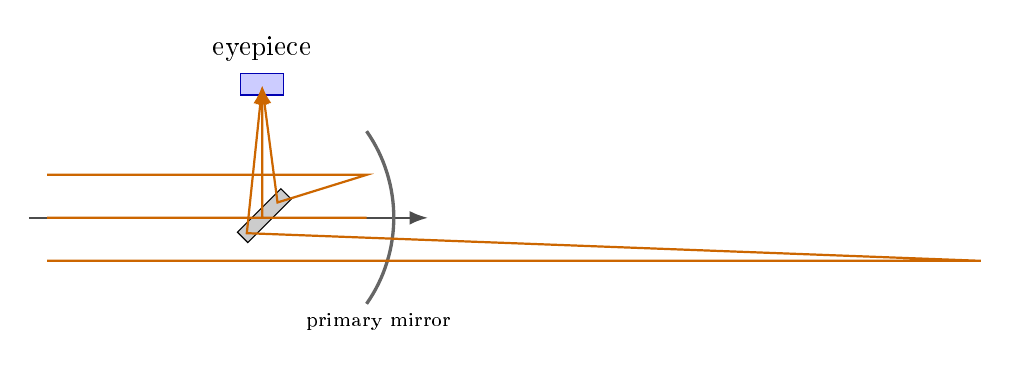
\begin{tikzpicture}[scale=0.78]
  \draw[axis] (-0.5,0)--(6,0);

  % primary mirror
  \draw[mirror] (5,-1.4) arc (-35:35:2.45);

  % flat secondary mirror
  \draw[fill=gray!40,draw=black,rotate around={45:(3.3,0)}]
    (2.85,-0.12) rectangle (3.85,0.12);

  % eyepiece / focal plane
  \draw[fill=blue!20,draw=blue!70!black]
    (2.95,2.0) rectangle (3.65,2.35)
    node[midway,above=5pt]{eyepiece};

  \coordinate (F) at (3.3,2.15);

  % rays: reflected by primary, intercepted at different points
  % on the secondary, then brought together in the eyepiece
  \draw[ray] (-0.2,-0.7) -- (15,-0.7) -- (3.05,-0.25) -- (F);
  \draw[ray] (-0.2, 0.0) -- (5, 0.0) -- (3.30, 0.00) -- (F);
  \draw[ray] (-0.2, 0.7) -- (5, 0.7) -- (3.55, 0.25) -- (F);

  \node[note] at (5.2,-1.7){primary mirror};
\end{tikzpicture}
\end{column}
\end{columns}

\pagebreak
\item \textbf{Cassegrain reflector}
\begin{columns}[T]
\begin{column}{0.47\textwidth}
\item A concave primary mirror and convex secondary mirror fold the optical path. The final focus lies behind the primary mirror.

\item This gives a long effective focal length in a compact tube.
\end{column}
\begin{column}{0.5\textwidth}
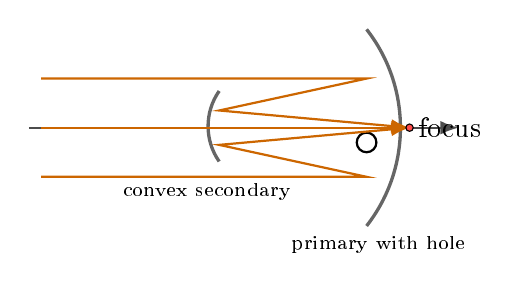
\begin{tikzpicture}[scale=0.78]
  \draw[axis] (-0.5,0)--(6.5,0);
  \draw[mirror] (5,-1.6) arc (-38:38:2.6);
  \draw[white,draw=black,thick] (5, -0.24) circle (0.16);
  \draw[mirror] (2.6,-0.55) arc (215:145:1.0);
  \foreach \y in {-0.8,0,0.8}{\draw[ray] (-0.3,\y)--(5,\y)--(2.6,{0.35*\y})--(5.7,0);} 
  \draw[fill=red!70] (5.7,0) circle (0.06) node[right]{focus};
  \node[note] at (2.4,-1.05){convex secondary};
  \node[note] at (5.2,-1.9){primary with hole};
\end{tikzpicture}
\end{column}
\end{columns}

\pagebreak
\item \textbf{Schmidt telescope / Schmidt camera}
\begin{columns}[T]
\begin{column}{0.47\textwidth}
\item A thin aspheric Schmidt corrector plate reduces spherical aberration from a spherical primary mirror.

\item \textbf{Purpose:} wide-field imaging with a relatively simple primary mirror.
\end{column}
\begin{column}{0.5\textwidth}
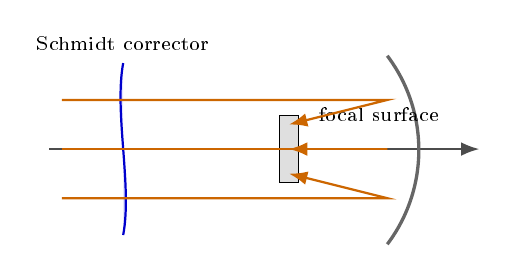
\begin{tikzpicture}[scale=0.78]
  \draw[axis] (-0.5,0)--(6.5,0);
  \draw[fill=blue!10,draw=blue!80!black,thick] (0.7,-1.4) .. controls (0.85,-0.6) and (0.55,0.6) .. (0.7,1.4);
  \node[above,note] at (0.7,1.45){Schmidt corrector};
  \draw[mirror] (5,-1.55) arc (-37:37:2.55);
  \draw[fill=gray!25,draw=black] (3.25,-0.55) rectangle (3.55,0.55) node[right=4pt,note]{focal surface};
  \foreach \y in {-0.8,0,0.8}{\draw[ray] (-0.3,\y)--(0.7,\y)--(5,\y)--(3.4,{0.5*\y});}
\end{tikzpicture}
\end{column}
\end{columns}

\pagebreak
\item \textbf{Ritchey--Chretien reflector}
\begin{columns}[T]
\begin{column}{0.47\textwidth}
\item A Ritchey--Chretien telescope uses a concave hyperbolic primary and a convex hyperbolic secondary.

\item \textbf{Advantage:} it corrects primary spherical aberration and coma, giving excellent wide-field astronomical imaging.

\item \textbf{Trade-off:} curved focal plane and more difficult fabrication/alignment.
\end{column}
\begin{column}{0.5\textwidth}
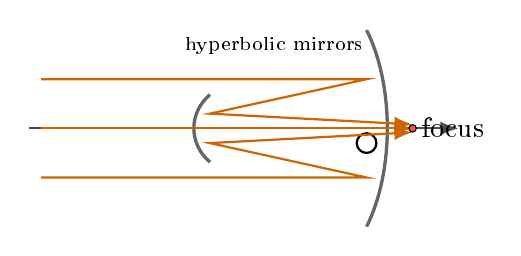
\begin{tikzpicture}[scale=0.78]
  \draw[axis] (-0.5,0)--(6.5,0);
  \draw[mirror] (5,-1.6) .. controls (5.45,-0.7) and (5.45,0.7) .. (5,1.6);
  \draw[white,draw=black,thick] (5, -0.24) circle (0.16);
  \draw[mirror] (2.45,-0.55) .. controls (2.1,-0.25) and (2.1,0.25) .. (2.45,0.55);
  \foreach \y in {-0.8,0,0.8}{\draw[ray] (-0.3,\y)--(5,\y)--(2.45,{0.30*\y})--(5.75,{0.08*\y});}
  \draw[fill=red!70] (5.75,0) circle (0.06) node[right]{focus};
  \node[note] at (3.5,1.35){hyperbolic mirrors};
\end{tikzpicture}
\end{column}
\end{columns}

\pagebreak
\item \textbf{Lens telescopes versus mirror telescopes}
\begin{tabular}{p{0.18\textwidth}p{0.36\textwidth}p{0.36\textwidth}}
\toprule
 & Refracting telescopes & Reflecting telescopes \\
\midrule
Main element & Objective lens & Primary mirror \\
Advantages & Sealed tube possible; stable alignment; high contrast; simple light path & No chromatic aberration; large apertures are practical; compact folded designs possible \\
Disadvantages & Chromatic aberration unless corrected; heavy large lenses; lens sag and absorption & Central obstruction; mirror coating aging; collimation and thermal effects \\
Best uses & Small high-quality visual telescopes, teaching, terrestrial viewing & Large astronomical telescopes, deep-sky imaging, professional observatories \\
\bottomrule
\end{tabular}
%\vspace{0.5em}
\pagebreak
\item \textbf{Final comparison:} Refractors are often mechanically simple and high contrast at small aperture. Reflectors dominate at large aperture because mirrors can be supported from behind and avoid chromatic aberration.

\end{itemize}
\end{frame}

% ----------------------------------------------------------------------------------------------------------------------------------------

\begin{frame}
%\frametitle{Minden jó, ha a vége jó}

\vfill
\begin{center}
\textbf{\huge The End}

\bigskip
Thank you for your attention!
\end{center}
\vfill
%\textbf{Acknowledgements} Thank you for the course materials for Szilárd~ZSÓKA and Zoltán~VARGA.
\end{frame}

\end{document}
